\documentclass[tikz,border=2pt]{standalone}
\usepackage{amsmath,amssymb}
\usepackage{tikz}
\usetikzlibrary{matrix,arrows.meta}

\begin{document}
% One simplex pivot: x_s enters, s_3 leaves (pivot element 1 in row s_3). The pivot row is
% normalised and subtracted from the other rows so that the x_s column becomes a unit column.
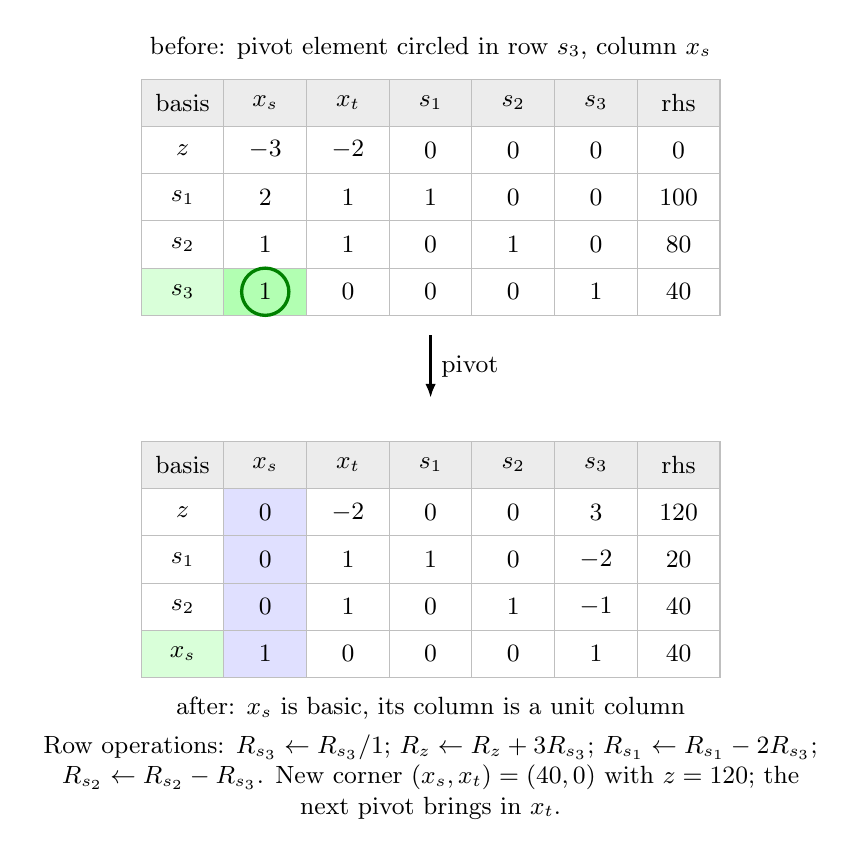
\begin{tikzpicture}[every node/.style={font=\small}, >={Latex[length=1.8mm]}]
	\matrix (A) [matrix of math nodes, nodes={minimum width=1.05cm, minimum height=6mm, anchor=center, draw=gray!50}, column sep=-\pgflinewidth, row sep=-\pgflinewidth] at (0,0) {
		|[fill=gray!15]| \text{basis} & |[fill=gray!15]| x_s & |[fill=gray!15]| x_t & |[fill=gray!15]| s_1 & |[fill=gray!15]| s_2 & |[fill=gray!15]| s_3 & |[fill=gray!15]| \text{rhs} \\
		z & -3 & -2 & 0 & 0 & 0 & 0 \\
		s_1 & 2 & 1 & 1 & 0 & 0 & 100 \\
		s_2 & 1 & 1 & 0 & 1 & 0 & 80 \\
		|[fill=green!15]| s_3 & |[fill=green!30]| 1 & 0 & 0 & 0 & 1 & 40 \\
	};
	\node[anchor=south] at (A.north) {before: pivot element circled in row $s_3$, column $x_s$};
	\draw[green!50!black, very thick] (A-5-2.center) circle (3mm);
	\draw[->, very thick] (0,-1.75) -- (0,-2.55) node[midway, right] {pivot};
	\matrix (B) [matrix of math nodes, nodes={minimum width=1.05cm, minimum height=6mm, anchor=center, draw=gray!50}, column sep=-\pgflinewidth, row sep=-\pgflinewidth] at (0,-4.6) {
		|[fill=gray!15]| \text{basis} & |[fill=gray!15]| x_s & |[fill=gray!15]| x_t & |[fill=gray!15]| s_1 & |[fill=gray!15]| s_2 & |[fill=gray!15]| s_3 & |[fill=gray!15]| \text{rhs} \\
		z & |[fill=blue!12]| 0 & -2 & 0 & 0 & 3 & 120 \\
		s_1 & |[fill=blue!12]| 0 & 1 & 1 & 0 & -2 & 20 \\
		s_2 & |[fill=blue!12]| 0 & 1 & 0 & 1 & -1 & 40 \\
		|[fill=green!15]| x_s & |[fill=blue!12]| 1 & 0 & 0 & 0 & 1 & 40 \\
	};
	\node[anchor=north] at (B.south) {after: $x_s$ is basic, its column is a unit column};
	\node[anchor=north, align=flush center, text width=10cm] at (0,-6.7) {Row operations: $R_{s_3}\leftarrow R_{s_3}/1$; $R_z\leftarrow R_z+3R_{s_3}$; $R_{s_1}\leftarrow R_{s_1}-2R_{s_3}$; $R_{s_2}\leftarrow R_{s_2}-R_{s_3}$. New corner $(x_s,x_t)=(40,0)$ with $z=120$; the next pivot brings in $x_t$.};
\end{tikzpicture}
\end{document}
